\section{Base Finite Volume Schemes}\label{sec:basefv}

Our computational results use two different finite volume schemes
to update the cut cell mesh, to show that SRD can be used in a
variety of situations.
We will refer to these as the base schemes. 
The  base scheme is applied to the entire mesh, including  
to the small cut cells, using the same time step $\Delta t$ for all cells.  
Since cut cells can have cell volumes that are
orders of magnitude smaller than the time step allowed by the full
cells, these will lead to instability without a stabilization algorithm.
SRD will be applied after each stage or step of the base scheme.

\begin{figure}
\begin{center}
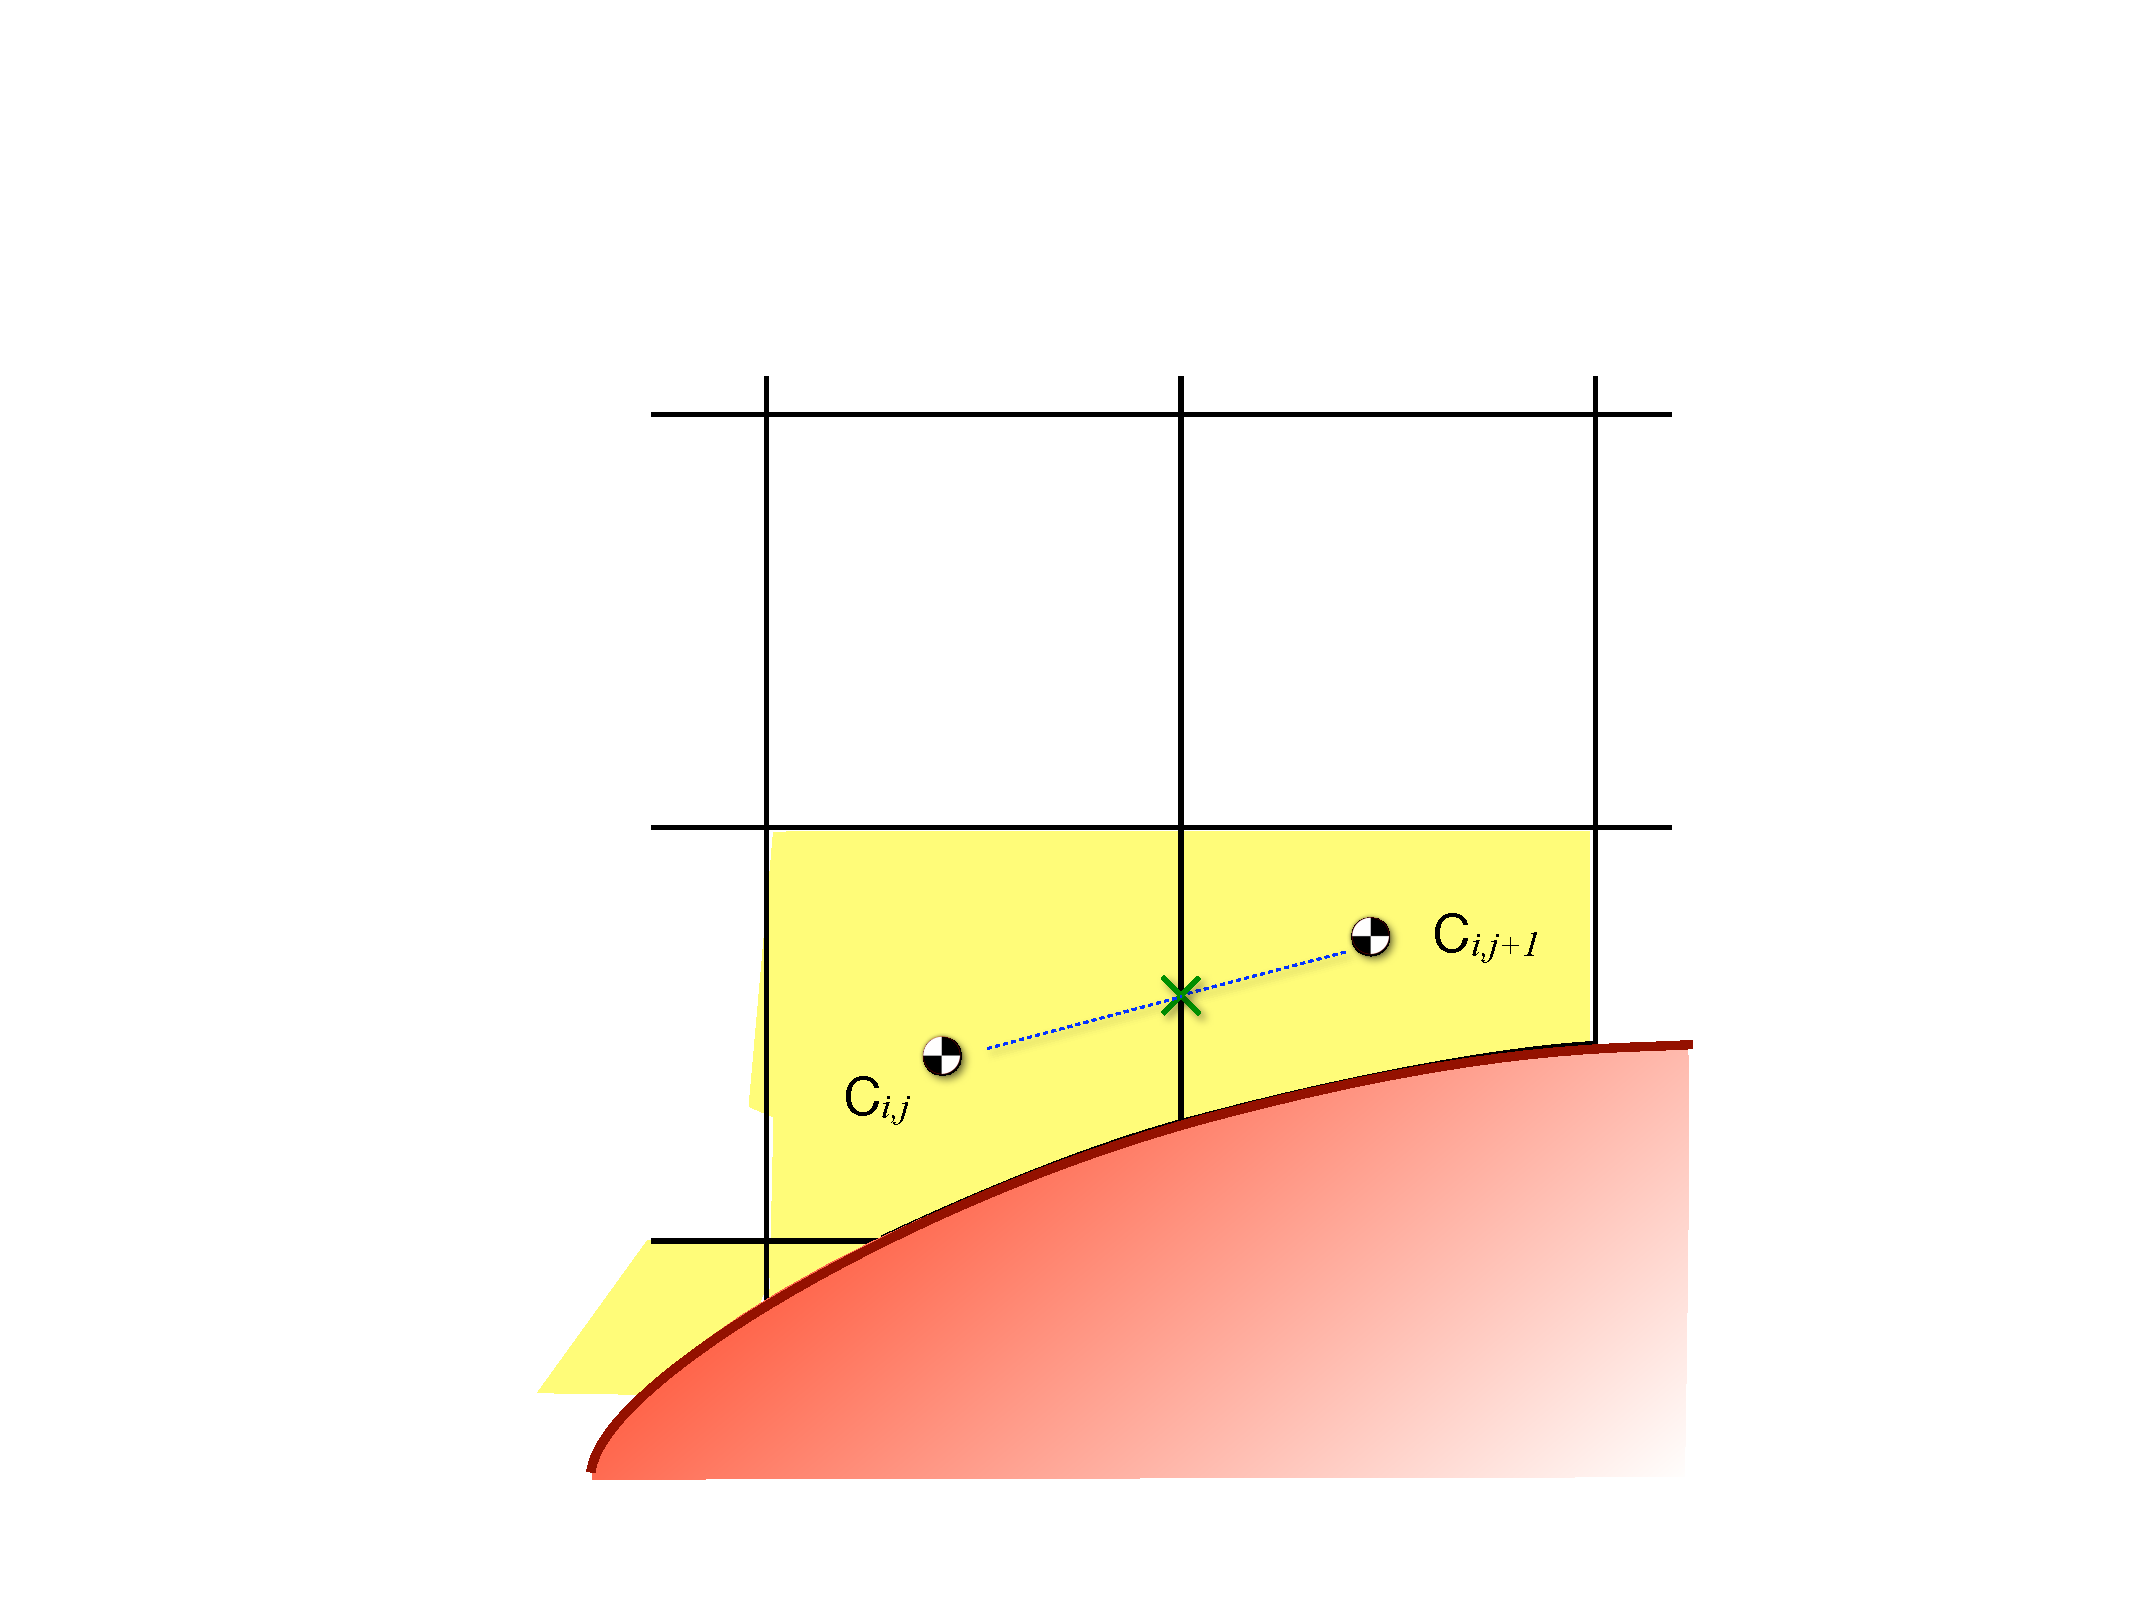
\includegraphics[width=3.0in]{figs/2dfig.pdf}
\caption{\sf Notation for mesh in two space dimensions. The cells shaded
in yellow are the cut cells.} 
\label{fig:2dfig}
\end{center}
\end{figure}

The question of computing gradients, and for problems with discontinuities limiting
those gradients, arises independently of which finite volume scheme is used. 
For the interior of the mesh when the stencil is completely regular (i.e. no cut
cells), standard schemes such as monotonicized central differencing can be 
applied, so we do not discuss this further.
For cut cells, we use a least squares gradient reconstruction algorithm which is
linearly exact.  We outline the gradient reconstruction, and
discuss two  limiting procedures for the cut cells in 
section \ref{sec:limit}. Our examples will always report which scheme and
limiter was used.


\subsection{Method of Lines approach}
The simplest scheme is to use a spatial discretization over the entire
mesh, and apply a Runge-Kutta scheme in time. This is a well-known
standard approach
on regular Cartesian meshes. It is adapted for the cut cells by
using the  least squares reconstruction of the gradient mentioned above, and one of
the limiters described in section \ref{sec:limit}.

The spatial reconstruction in the cut cells is no longer
coordinate-aligned, and is easily adapted to  
include both $x$ and $y$ components of the gradient to 
reconstruct to the midpoint of the cell edge. 
Figure \ref{fig:2dfig}  indicates this face location with a green $\times$.
Note that the time step restriction that results from the von Neumann 
stability analysis of this scheme applied to the linear advection equation is  (AG -
TRUE or this is for positivity?)
\begin{equation}
\Delta t \,  \max\left(\frac{u}{\Delta x},\frac{v}{\Delta y}\right) \leq \frac{1}{2} ,
\end{equation}
where $(u,v)$ is the propagation velocity.  

\subsection{MUSCL scheme}
The MUSCL scheme is a one step method that is second order accurate in
time. A series of MUSCL schemes  was originated by van Leer 
\cite{vanleer:muscl}. The version we use\footnote{Thanks to Phil 
Colella for the original Cartesian mesh code and for helpful discussions on the shear
layer instability and artificial viscosity.}
is due to Colella \cite{Colella:Unsplit}.
The method is briefly sketched here so that we can describe how it was
adapted for cut cells. 

On a regular cell $(i,j)$ the interface values on the 
faces are computed at the half-step in time, and the left and right states
are passed to a Riemann
solver to compute the fluxes.
Using a Taylor series in space and time to second order around the
cell center, and using the equation to replace the derivative in time,  gives
\begin{equation}\label{taylor}
\begin{split}
q_{i+1/2,j}^{n+1/2} & = q_{i,j}^n + 
              \frac{\Delta t}{2} \frac{\partial q_{ij}^n}{\partial t} + 
              \frac{\Delta x}{2} \frac{\partial q_{ij}^n}{\partial x} \\[.08in]
            &  = q_{i,j}^n + \frac{\Delta t}{2} 
            (-\frac{\partial f_{ij}^n}{\partial x} -
             \frac{\partial g_{ij}^n}{\partial y})  +
             \frac{\Delta x}{2} \, \frac{\partial q_{ij}^n}{\partial x} \\[.08in]
            &  = q_{i,j}^n - \frac{\Delta t}{2} \, 
             \frac{\partial g_{ij}^n}{\partial y}  -
            ( \frac{\Delta t}{2} 
            \frac{\partial f_{ij}^n}{\partial q} -
             \frac{\Delta x}{2} ) \,\frac{\partial q_{ij}^n}{\partial x} . \\[.08in]
\end{split}
\end{equation}
After discretization, this will become the left state of the right interface
of cell $(i,j)$.

In the original method, the term $\partial g / \partial y$ is computed by solving Riemann
problems in the vertical direction,  evaluating the flux $g$, and computing the
difference in fluxes divided bt $\Delta y$.
Since this only needs to be done to first order accuracy (the term is multiplied
by $\Delta t$)  no reconstruction to the cell edge  in the transverse 
direction was necessary,
and differencing the edge fluxes was appropriately cell-centered.
(For more details the reader is referred to \cite{Colella:Unsplit}.)
Note that it is this transverse derivative that provides the so-called corner coupling,
giving the MUSCL scheme a stability limit of
\begin{equation}
\label{eqn:bigcfllimit}
\Delta t \, \max \left (\frac{u+c}{\Delta x} , \frac{v+c}{\Delta y} \right) < 1
\end{equation}

At the cut cells this procedure will no longer work.   We make two modifications to the
computation of the transverse derivatives. First,
the solution is reconstructed to the edge midpoint  for the transverse Riemann problem.
This takes care of the situation where a full cell is adjacent to a cut cell, and
the transverse flux would not be properly centered. This is the situation
in figure \ref{fig:2dfig} for cell $(i,j+1)$, for example.
Secondly, most cut cells will not have a flux on the other side to form a
transverse derivative, for example cell $(i+1,j)$. Even for cell $(i,j)$ is would
be difficult to find a location where the vertical fluxes could be accurately differenced.
For these cut cells, the transverse derivative term is handled by instead computing
$ \partial G / \partial y \, = \,  \partial G / \partial q \times \partial q / \partial y$,
as with the horizontal fluxes. This is linearly exact in the cut cells, 
if the gradients themselves are.

As remarked above, it is the transverse derivatives that allows for the larger time
step given in \eqref{eqn:bigcfllimit}.
However, in the neighborhood of a shock the derivatives will be limited, and
possibly set to zero.
If these terms were not used  in the volume mesh, the time step would be reduced to 
\begin{equation}
\Delta t \, \left (\frac{u+c}{\Delta x} + \frac{v+c}{\Delta y} \right) < 1
\end{equation}
which could be as small as half the larger limit in eq. \eqref{eqn:bigcfllimit}.
However, as shown in \cite{mjb:stability2} for one space dimension, 
boundary cells can have
a local {\em cfl} number that is up to twice the stable {\em cfl} of the regular
mesh and the overall scheme remains stable.  We have not found any stability
problems due to limiting of this term.  

The multi-dimensional MUSCL scheme due to Colella has several additional
features to robustly handle strong shocks, such as not including terms in the
interface state from characteristics that propagate away from the interface. These
steps do not change at the cut cells, so are not discussed here.  The
trickiest term to adapt to cut cells was an artificial viscosity 
added to each flux with a
coefficient proportional to the negative divergence of the flow.  The original
code used a very large stencil to compute this divergence. We instead use a local 5
point centered stencil to compute $u_x$ and $v_y$, and take the max over a 3 by 3
neighborhood, so that cut cells get this dissipation too.

\subsection{Gradient reconstruction and limiting for irregular
cells}\label{sec:limit}

Both base finite volume schemes have to compute a gradient on cut cells, and for
problem with shocks, limit it. 
We use the least squares approach, standard for unstructured meshes,
to compute a gradient on the cut cells, and one adjacent cell.
Cells that are two away from a cut cell
can use any limiter with a standard stencil size. 

A linear reconstruction of the solution in cell $(i,j)$
either a cut cell or cell with an irregular stencil, is of the form
\begin{equation}
u(x,y) = u_{ij}^n + \sigma_{x,i,j} \,(x-x_{i,j}) +
                     \sigma_{y,i,j}\,(y-y_{i,j}),
\label{eqn:lls}
\end{equation}
where $(\sigma_{x,i,j},\sigma_{y,i,j})$ is the gradient in 
cell $(i,j)$, and $(x_{i,j},y_{i,j})$ is the cell centroid. The least squares procedure
finds the gradient that minimizes the $l_2$ residual when evaluating  $u(x,y)$
at a neighboring cell centroid. We typically use vertex neighbors to form the matrix,
since it can happen that a cell only has two edge neighbors (e.g. cell $(i,j-1)$ in
Figure \ref{fig:2dfig}.  This procedure is linearly exact.  

For problems with discontinuities, the gradient will need to be limited
to prevent overshoots and retain positivity for quantities like density and
pressure.
We use two possible methods, and compare them in the some of the 
computational examples.
The simplest procedure  is to use the Barth Jespersen (BJ) limiter
\cite{barth-jespersen}. 
This is a scalar limiter: both $\sigma_x$ and $\sigma_y$ are reduced by
the same scalar that prevents new extrema.  The BJ limiter  can also be
used in the interior of the mesh, and so is closer to the base scheme. 

To limit using BJ, we compute the minimum and maximum values over the
reconstruction stencil $R_{i,j}$, i.e.
\begin{equation}
     m_{i,j} = \max_{k \in R_{i,j}} {u}_k^n \text{ and } M_{i,j} = \max_{k \in R_{i,j}} 
     {u}_k^n.
\label{eqn:bj}
\end{equation}
The reconstructed gradient on cell $(i,j)$ is limited by a non-negative 
scalar $\alpha \in [0,1]$, so that the linear function becomes 
\begin{equation}
     u(x,y) = {u}_{i,j}^n + \alpha [{\sigma}_{x,i,j} ( x -  x_{i,j}) \, 
   + {\sigma}_{y,i,j}( y -  y_{i,j})].
\end{equation}
The scalar $\alpha$ reduces the gradient such that when ${u}(x,y)$ 
is evaluated at the centroids of the neighborhoods in $R_{i,j}$ it
lies between $m_{i,j}$ and $M_{i,j}$.
It is given by
$$
\alpha = \max\left(0,\min_{k \in R_{i,j}} \alpha_k \right),
$$
where
\begin{equation}
    \alpha_k = \begin{cases}
    \frac{{u}( x_{k},  y_{k}) - {u}_{i,j}^n}{M_{i,j} -
    {u}_{i,j}} \quad  \text{  if  } {u}( x_{k},  y_{k}) - {u}_{i,j}^n \geq 0,\\[.08in]
     \frac{{u}( x_{k},  y_{k}) - {u}_{i,j}^n}{m_{i,j} -
     {u}_{i,j}^n}  \quad \text{  if  } {u}(x_{k}, y_{k}) - {u}_{i,j}^n < 0.
    \end{cases}
\end{equation}
With this limited gradient, the reconstruction for each cell satisfies a
local maximum principle
\begin{equation}
m_{i,j} \le u(x,y) \le M_{i,j} \quad \forall k \in R_{i,j}
\end{equation}

The other limiter we test is the LP limiter 
\cite{May_Berger_LP}. This is a vector limiter, where both components of
the gradient are reduced by the smallest amount that still satisfies some
constraints. An small LP problem is solved to obtain these quantities.
The LP limiter retains more of the original gradient
and is less diffusive than the BJ limiter at cut cells, 
but is roughly twice the computational cost.
We will always include which limiter is used
in the computational results.  

